%!TEX root = thesis_main.tex

\chapter{Introduction}\label{ch:intro}
Write once I am finished with the rest of the introduction so I can summarize it in a sort of "abstract." 

\section{Motivation} \label{intro:motivation}

As robotic applications flourish in our modern world, robotic systems are pushing to be smaller, lighter, and more efficient. 
Therefore the need for effective torque reduction in small, compact, and weight efficent packages increases. 
The prevelance of robots in development throughout the world is striking. 
Everyone can recognize the famous robots like the great work out of Boston Dymamics with Big Dog, Atlas, spot, and many others \cite{ref/boston_dynamics}, or the Honda's Asimo \cite{ref/asimo}.  
However, this is a very small subset of the robots that are currently on the market now. 
There are a huge number of 6 DoF manipulators being constructed and sold like the UR series from Universal Robotics, the industrial arms from KUKA, ABB, Fanuc, DENSO and even small servo operated arms available for hobbiests. 
Nearly every one of these larger robots has some sort of gear reduction between the motor and the output of each joint, therefore, the expansion of the available technologies for these reductions is clear as robotics push further and further into our factories, cities, and everyday lives. 

These technologies also translate directly to the work being done by NASA in the area of robotics. 
NASA is active in many types of robotic systems including humanoid robotics, rovers, and satellite technologies. 
The two primary examples of NASA's robotic technologies comes from their humanoid robots, Robonaut 2 (R2) \cite{ref:r2}, and Valkyrie \cite{valkyrie} as well as the rover technologies like the Mars rovers, most recently Curiosity \cite{ref:curiosity}, the manned rover prototypes \cite{ref:rover}, and lunar rovers \cite{ref:RP}. 
These robotic systems share many of the same design challenges as those found in industry, as well as additional challenges due to the extreme environments they travel to. Therefore, the advancement of actuator technology is especially important in these areas as NASA strives to go further into the solar system with humans and robotic systems. 

\begin{figure}[!b]
   \centering
   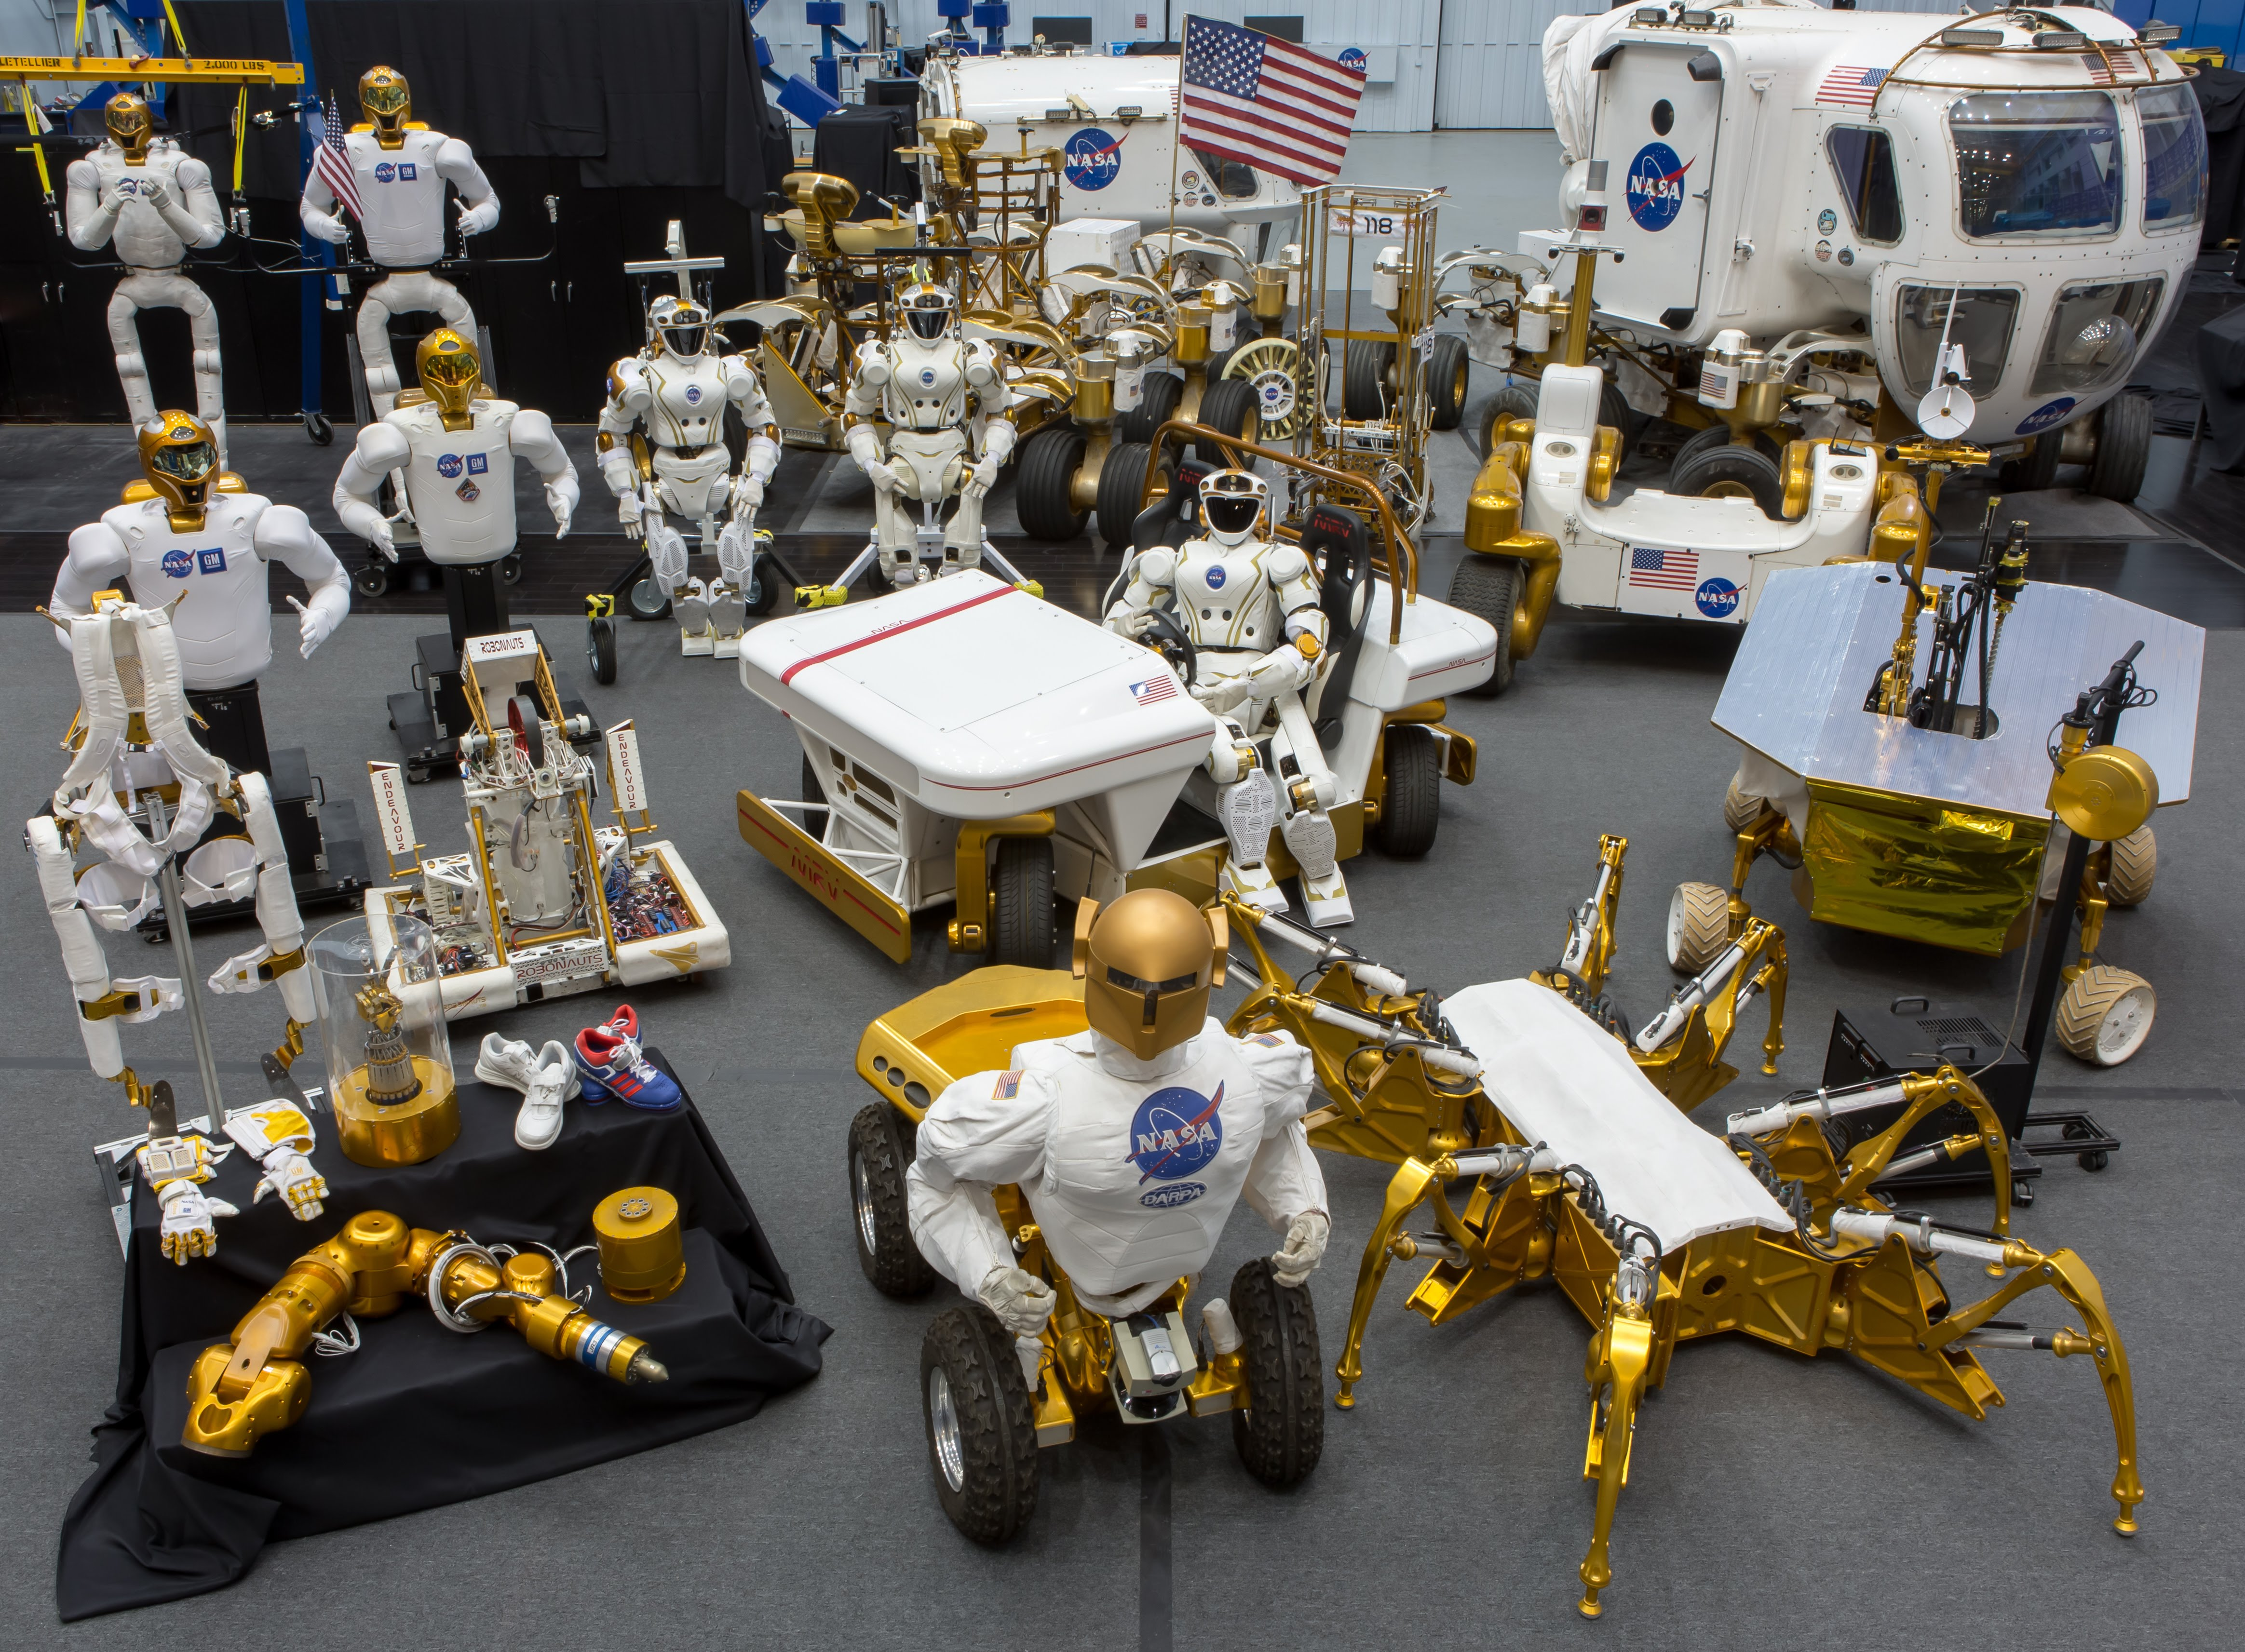
\includegraphics[width=0.7\linewidth]{fig/robot_collage}
   \caption{insert a collage picture of the above mentioned NASA robots}
   \label{fig/robot_collage}
\end{figure}


Generally, these robots must balance a number of factors based on their specific design goals, these usually involve efficiency, strength, speed, and precision in some combination. 
With these aforementioned goals comes the trade of the actuator design for where factors such as backlash, backdriveability, efficiency, torque output, speed, and packaging. 
Reductions for these systems are usually one of three types: planetary gearsets, belt drives, and harmonic drives. 
Each of these drives has their own advantages. 
Planetary gearsets can be customized to meet a desired reduction, are commonly produced, and run very efficienctly.
Belt drives share many of the benefits of planetary gearsets, and have very minimal backlash, but take more volume for a similar reduction. 
Harmonic drives are generally much more compact for the reduction they provide and have no backlash as well, but run less efficiently than the other two. 
Due to the higher reduction per volume, harmonic drives are usaully the reduction of choice in robotic actuator design in cases where compact design is favored over efficiency.

\begin{figure}[!b]
   \centering
   \includegraphics[width=0.7\linewidth]{fig/actuator_type_collage}
   \caption{insert a picture collage of other types of reducers}
   \label{fig:reducer_collage}
\end{figure}

There exists a fourth option to add to this list however, cycloidal drives. 
Cycloidal drives provide a high reduction per volume similar to a harmonic drive, but can provide a higher specific torque than a harmonic drive. 
Cycloidal drives do generally have backlash, so these designes cannot replace a harmonic drive in every situation, but a cycloid does provide an interesting option in design cases where high reduction and high torque in a small package is necessary, and a small amount of backlash is acceptable. 
However, these cycloidal drives are not currently in common use even with these distinct advantages over a harmonic drive due to the lack of information on their actual in-use characteristics. 

\section{Harmonic Drives} \label{intro:harmonic}

The concept of a harmonic drive was proposed as early as 1959 by Walton Musser \cite{ref:harmonic_original} and have been further improved in design and implementation through the years. The original harmonic drive patent has been cited in over 200 subsequent patents according to Google patent search. These drives were first used in spaceflight applications in 1971 as the primary drive motors for the Apollo Lunar Rovoers \cite{ref:harmonic_apollo}. A notable adapation of this patent that lead to the current common method of manufacturing harmonic drives was issued by Harmonic Drive in 1989 \cite{ref:harmonic_drive_co} which lead that company to be one of the primary producers of harmonic drive technologies until recently when the patent expired. 

\begin{figure}[!b]
   \centering
   \includegraphics[width=0.7\linewidth]{fig/harmonic_cartoon}
   \caption{Insert cartoon of harmonic drive}
   \label{fig:harmonic_cartoon}
\end{figure}

Harmonic drives utilizes the deflection of metal to induce motion. The harmonic drive consists of three main pieces, a wave-generator, a flex cup, and a circular spline (Fig \ref{fig:harmonic_cartoon}). The wave generator is a slightly elliptical shape that is mounted to the output of the motor. This is inserted into the flex cup, a thin metal cup with T\textsubscript{flex} teeth that allows some flexing as the elliptical wave-generator rotates through it. Finally, the flex cup and wave-generator sytem is inserted into the circular spline, a thicker, stiff piece of metal that has a different number of teeth (T\textsubscript{circ}) than the input. As the wave-generator rotates inside the flex cup, pushing the walls out, it slowly works its way into the next available tooth, creating a counter-rotation of the flex-cup which is harnessed as the output of the system. This results in high ratios in the form of 

\begin{equation} \label{eq:0}
ratio = \frac{T_{flex} - T_{circ}} {T_{flex}}.
\end{equation}

Harmonic drives have two primary advantages in their use. First, harmonic drives can accomplish high reductions in a smaller volume than a typical planetary reduction. Second, harmonic drives have no backlash, allowing precision control with no additional considerations that must be taken. However, these positives come at a cost as well, the efficiency of harmonic drives is generally substantially lower than their planetary counterpart and varies drastically with temperature. In \ref{fig:harmonic_eff} a reproduction of the efficiencies quoted in the harmonic drive manual can be seen for reference. These efficiency results from the data sheet can be further supported for space applications by the research of Schafer et. al. \cite{ref:harmonic_space_lube} and \cite{ref:harmonic_performance}. Even with these disadvantages, harmonic drives are still the primary source of high reduction ratios in robotic platforms today. 

\begin{figure}[!b]
   \centering
   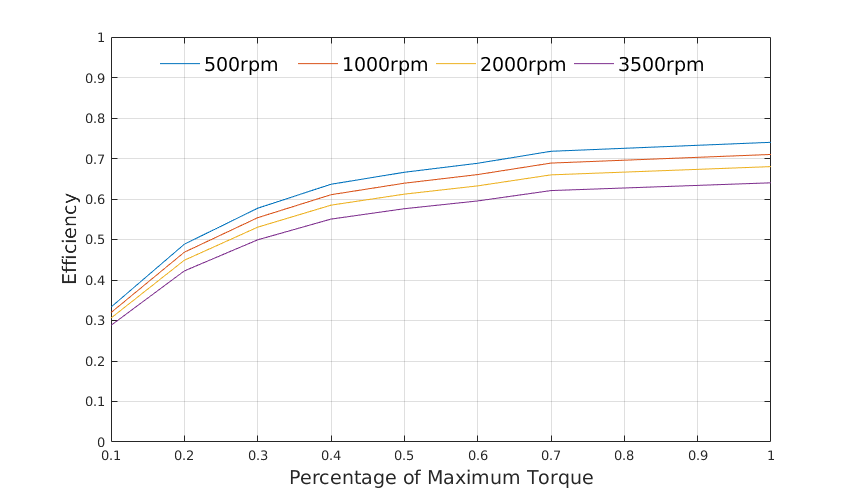
\includegraphics[width=0.7\linewidth]{fig/harmonic_eff}
   \caption{insert a reproduced graph from the harmonic drive manual for the drive that's comparble to the 1 stage }
   \label{fig:harmonic_eff}
\end{figure}

\section{Cycloidal Drives} \label{intro:cycloid}

An alternative technology for high reductions in small packages comes in the form of cycloidal drives. The original concept for the induced motion seen in a cycloidal drive pre-dates harmonic drive. The original patent for the idea was filed by Hoist in 1931 \cite{cycloid_original}. However, the proliferation of this technology did not accelerate at the same speed as the harmonic drive, with this original patent only receiving 12 citations. A large development in the technology came with the invention of Rudolf Braren in 1977 \cite{ref:cycloid_one_stage} who proposed the concept and equations necessary for the common method of constructing cycloids that is used today. In 1981, Keith Rodaway patented the concept of a pinwheel reduction \cite{ref:cycloid_pinwheel}, which allowed much more compact designs of the cyloidal system. This compact design allows is the driving design for the compact, high torque density and high specific torque designs that are discussed in this work.

The premise of this design leverages a plate, referred to as the wobble plate, with lobes interacting with pins in the housing designed using trochoidal motion being spun on an eccentric shaft with a bearing.
This eccentric lobe to pin interaction induces a counter-clockwise motion of the plate that is harnessed with the interior pins as the output of the mechanism (seen in Fig \ref{fig:cycloid_cartoon}) with the reduction equation \ref{eq:single_stage_ratio}.

\begin{equation} \label{eq:single_stage_ratio}
Z = \frac{Z_{lobes}} {Z_{pins} - Z_{lobes}}
\end{equation}

This geartrain design has been used in industry for high torque, high shock load applications for many years including companies like Natbesco Motion Control and Onvio.
However, in many of these applications, many or all of the interacting surfaces like the housing pins and output pins use needle roller bearings to transmit load.
This allows for higher efficiency and load carrying capability, but it also increases mass and volume.
In the robotic industry, groups are striving to reduce the mass and volume of these actuators while still achieving high reduction and load capabilities.
One method for reducing mass is eliminating the rolling elements at the interaction points between the wobble plate, housing pins, and output pins.
This allows for very compact and strong designs to be considered, but leaves the potential for larger losses and shorter system lifetime. The details of this design will be presented in \ref{ch:design_1s} and the efficiency of an example compact design will be presented in \ref{ch:design_2s}. 

\begin{figure}[!b]
   \centering
   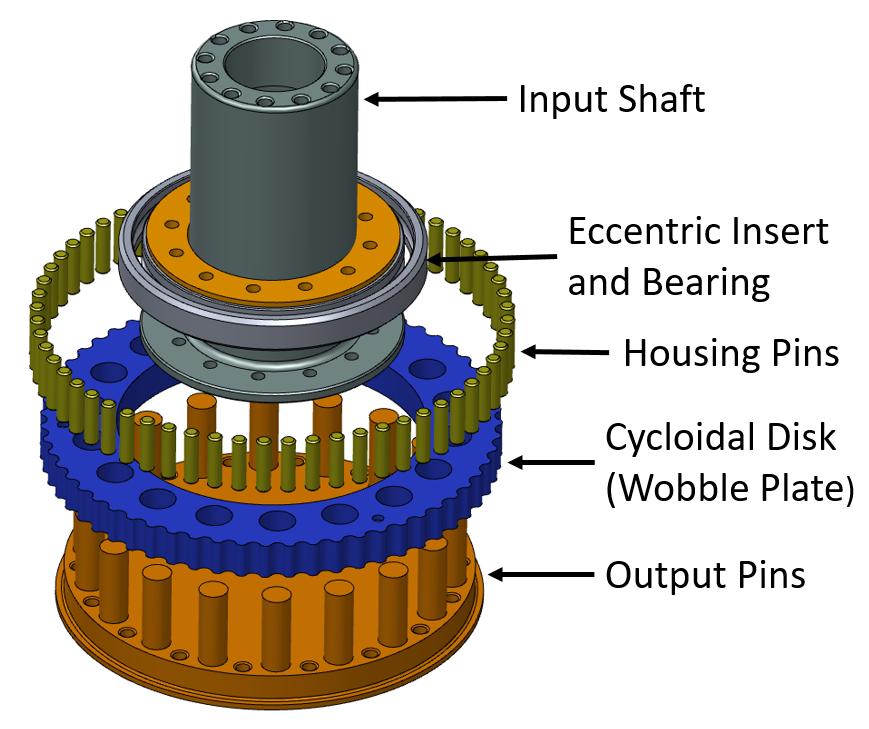
\includegraphics[width=0.60\linewidth]{fig/cycloid_cartoon_v2}
   \caption{Simple rendering of the key elements that create a cycloidal drive.
   A drive shaft spins a cycloidal disk (wobble plate) via an eccentric circle.
   The wobble plate reacts against the housing pins to create a counter-rotation, harnessed by the output pins. TODO -- add labels for number of teeth}
   \label{fig:cycloid_cartoon}
\end{figure}

More recently, authors have proposed designs that create a ``two-stage'' reduction using the cycloid profile. Instead of a typical two stage reduction system in which the output of one cycloid reducer drives the eccentric shaft as the input of the second reducer, the counter-rotation of the wobble plate is harnessed and directly passed to a second wobble plate that interacts with the lobes in the housing that are free to rotate \cite{ref:new_two_stage}. This design allows for more compact high reduction systems with a reduction defined in eq. \ref{eq:two_stage_ratio} \cite{ref:two_stage_tooth_mod}. The details of this design with be outlined more completely in \ref{chapter3:design}.

%put 2 stage equation
\begin{equation} \label{eq:single_stage_ratio}
Z = \frac{Z_{lobes}} {Z_{pins} - Z_{lobes}}
\end{equation}

Many works have been presented on the subject of the theoretical design of these cycloidal drives \cite{ref:on_the_lobe} \cite{ref:hwang_hsieh}, designing with machine tolerances \cite{ref:design_and_application}, contact and stress analysis \cite{ref:li}, and performance characteristics such as torque ripple and backlash \cite{ref:hsieh_traditional} \cite{ref:hsieh_dynamics} as will be presented in Section \ref{design}.
These works lay a solid foundation for a designer, providing the equations and design considerations for a cycloid.
Still, there is a need to present in-use characteristics to support the theoretical calculations and models.

Theoretical cycloid efficiencies have been reported in the 88-98\% range \cite{ref:Malhorta}, \cite{ref:unified_approach}.
More recently, Sinsinger and Lipsey reported experimentally determined efficiencies for fused roller designs (42.3\%) and pin designs (71\%) based on 80 minutes of run-time \cite{ref:cycloid_vs_harmonic}.
The distinction between a fused roller and pin design comes in the design of the housing.
In a fused design, the input pins are machined as part of the housing, and in a pin design, pins are inserted to ride in the housing, allowing relative motion.

Hsieh verified the stress present in the drives in simulation and in-use which demonstrated lower stress levels and torque ripple when using fused rollers \cite{ref:hsieh_dynamics}.
These two results leave an open trade to designers if stress and torque ripple need to be minimized versus maximizing efficiency.

The previous work in this area lays a foundation of understanding for the construction and theoretical design of a single stage cyloidal drive, but there is a gap in the literature when it comes to in-use efficiency and lifetime of these devices. The benefits of designs like this are clear, but under-utilized in the robotic community. Additionally, the concept for a two-stage cycloid has been presented, but is lacking in the necessary design equations to produce compact two-stage cycloids. 

\section{Actuator System Motivation} \label{intro:projects}

\section{Contribution} \label{intro:contribution}

\section{Thesis Outline} 
